\documentclass{CFD2010paper}

%\usepackage{graphicx}
\usepackage[pdftex]{graphicx,color}

\title{PARAMETRIC STUDY OF A MULTISCALE FLUIDIC SYSTEM\newline
USING A HYBRID CFD-MD APPROACH}

\author{Soon-Heum Ko$^{\dag}$, Nayong Kim$^{\dag}$, Dimitris E. Nikitopoulos$^{\dag\dag}$, Dorel Moldovan$^{\dag\dag}$ and Shantenu Jha$^{{\dag},*}$}

\heading{S.-H. Ko, N. Kim, D. Nikitopoulos, D. Moldovan, and S. Jha}

\address{
$^{\dag}$Center for Computation and Technology,\\
Louisiana State University, 216 Johnston Hall, Baton Rouge, LA 70803\\
e-mail: \{sko,nykim,sjha\}@cct.lsu.edu
\\
$^{\dag\dag}$Department of Mechanical Engineering,\\
Louisiana State University, Baton Rouge, LA 70803\\
e-mail: \{meniki,moldovan\}@me.lsu.edu
\\
$^{*}$Contact Author}


\keywords{CFD (Computational Fluid Dynamics), MD (Molecular Dynamics), Hybrid CFD-MD Approach, Pseudo Compressibility, LAMMPS}

\abstract{
These days, with the emphasis on accurately solving the micro-scale fluid systems for the bio-fluidic product design, numbers of researches are accomplished using a hybrid CFD/MD approach. According to their approaches, the macroscopic flow characteristics are captured by a continuum hypothesis and low-speed flow regions are solved by a particle dynamics. By applying this method, the intermolecular effect on macroscopic flow can be accurately predicted with the reasonable efficiency. Meanwhile, we see some issues need to be clarified: (1) how we will set up hybrid conditions (layer size, sampling duration and interval) to minimize the particular velocity fluctuation to continuum domain, (2) whether current numerical techniques can be directly applied to naturally unsteady flow, and (3) whether current approach can be directly applied to solve moderate flow in larger system.

We use an in-house incompressible CFD code and a famous LAMMPS MD package and apply a hybrid scheme to these numerical solvers. We first solved the stationary flow with the same system size using MD package. This gives us the innate velocity fluctuation in the system and we can figure out the appropriate hybrid condition from this data. This hybrid condition is applied to validation and application problems. We validated our solution package by solving Couette flow and simulated the Stokes boundary layer problem, which concludes us that current hybrid scheme can be directly applied to solve naturally unsteady flow.

%By definition, hybrid simulation can expect more accurate solution than conventional CFD techniques and better efficiency than MD simulations. Meanwhile, we see some issues need to be clarified: (1) how we will set up hybrid conditions (layer size, sampling duration and interval) to minimize the natural velocity fluctuation by particle dynamics to continuum domain, (2) whether current numerical techniques can be directly applied to naturally unsteady flow. This motivates us to analyze the velocity fluctuation pattern in MD simulation to choose the best hybrid conditions for specific system, and apply the hybrid approach to naturally unsteady problem (Stokes boundary layer problem). An in-house incompressible CFD code and a famous LAMMPS MD package are used as baseline codes and hybrid schemes are applied on these numerical solvers. We start from the stationary flow simulation using MD package, which can give us the innate velocity fluctuation in that system. The appropriate hybrid condition acquired from this data is applied to validation and application problems. We validated our solution package by solving Couette flow and simulated the Stokes boundary layer problem, which concludes us that current hybrid scheme can be directly applied to solve naturally unsteady flow.

}



\begin{document}
%\maketitle



\newpage

\section{INTRODUCTION}
These days, with the emphasis on accurately solving the micro-scale fluid systems for the bio-fluidic product design, numbers of researches are accomplished using a hybrid CFD-MD approach$^{\cite{Thompson},\cite{Nie},\cite{Yen},\cite{Steijl}}$. In a word, a hybrid CFD-MD approach can be defined as adopting the continuum hypothesis in capturing macroscopic flow features while solving low-speed flow regions - whether it is near the stationary wall or not - by considering atomistic intermolecular interactions. CFD can accurately predict flow properties on conventional moderate/large size fluid domains, but is intrinsically impossible to reflect characteristics of surrounding solid materials. While MD can provide atomistic level resolution of interactions between particles, it becomes computationally demanding as the size of simulated system grows. The hybrid approach provides a good balance between computational cost and atomistic details/resolution.

An example of the macroscopic flow changes due to different atomistic interaction in the infinitesimal region is presented in Fig.~\ref{MD_Solution}. In this molecular dynamic simulation, different slip ratio between wall and fluid particle leads to the change in velocity gradient. In macroscopic point of view, molecular dynamic simulations describe the same flow physics as the continuum hypothesis. In microscopic level, it can represent the molecular interaction and the resulting changes which computational fluid dynamics cannot present. This evaluates the necessity to consider intermolecular effect on CFD solution procedure. Meanwhile, this result also shows an important issue in coupling continuum approach and molecular dynamics. The velocity fluctuation due to the innate molecular vibration is not what CFD can describe, thus suitable control of this fluctuation on domain interface is highly required.

%
\begin{figure}[ht]
\centering
\includegraphics[width=0.9\linewidth]{MD_Solution.pdf}
\vskip-0.2cm
\caption{Steady Couette Flow Solution by Pure Molecular Dynamic Simulation; In normal condition (with the unique potential well depth between flow particle and surface material, denoted by $\epsilon$), the solution by MD is identical to the result of continuum approach. In hydrophobic case (smaller $\epsilon$) the fluid shows a slight slip on the wall, while the fluid particle strongly attempts to stick to the wall in hydrophilic case (bigger $\epsilon$).}
\label{MD_Solution}
\end{figure}



Though the idea is novel and the approach is well refined, still a lot of issues are remained on the hybrid CFD-MD simulation. First, it is nearly impossible to incorporate distinct CFD and MD codes under the umbrella of a single tightly-coupled application, considering very different computational kernels (one could be mesh-based, the other unstructured particle simulations) with very different computational time-scales. Even in case hybrid interfaces and schemes are accurately implemented on CFD and MD packages, coupling parameters setup is another critical issue. Layer size of data exchange zone with its position, sampling duration and the interval are major factors which affect the accuracy of coupled solution. Controlling/managing the operation flow of individual (yet coupled) codes within the computer system raises additional computer scientific issues including co-scheduling and load balancing, which has been discussed in detail in Ref.${\cite{CCGrid}}$.
% which is beyond the scope of this paper. Detailed discussion on computational issues are referenced in ${\cite{CCGrid}}$.
%(Issues of coupled simulation in view of computer science - 'though not to be discussed in this paper, it would be valuable to briefly introduce major computer scientific issues in running this coupled simulation.... detailed discussion can be found in Ref. CCGrid paper'; 1 paragraph)\\

The current paper focuses on implementing hybrid interface on reliable CFD and MD codes and applying this coupled package on the simulation of multiscale application problems. We begin the next section with an outline of the basic motivation and concept of coupled simulations. Numerical details of individual code and implementation of hybrid scheme are presented in the next Section. Validation of coupled simulation package and its application to other problems follow in Section 4. Couette flow simulation and Stokes boundary layer problems are conducted on two different system scales. Hybrid layer size and sampling duration along with sampling interval, are discussed. The summary of our work and the future plan are expressed in Section 5.



\section{HYBRID CFD-MD SIMULATION APPROACH}

The study of microfluidic mechanism including from nanoscale fluidic system to continuum one has been recently developed using hybrid CFD-MD method. The hybrid method is taking the advantage of each atomistic and continuum descriptions adopting information exchange based on constrained equation of motion over the overlap region$^{\cite{Thompson},\cite{Nie},\cite{Yen},\cite{Steijl}}$. Modification for mutual flux exchange across the domain boundary has been proposed$^{\cite{Flekkoy},\cite{Wagner}}$ and more studies about the flux exchange scheme$^{\cite{Hadjicon1},\cite{Hadjicon2}}$, coupling parameters$^{\cite{Wang}}$ have been accomplished. However, more challenging point of view are still remaining such as extreme physical domain condition, explicit time duration of passing information, the region for taking the statistics of atomistic averaging and others.

The hybrid CFD/MD approach is a simulation method which adopts the continuum hypothesis in capturing macroscopic features of a flow-field and details atomistic
intermolecular interactions on interfaces of different materials by using the MD approach. CFD can accurately predict flow properties on conventional moderate/large size fluid domains, but is intrinsically
impossible to reflect characteristics of surrounding solid materials within a interfacial region. While standard classical MD can provide atomistic level resolution of interactions between particles, it becomes computationally demanding as the size of simulated system grows. So, neither method is suitable for solving a mesh-scale fluid system where the viscous effect dominates the flow characteristics but macroscopic features are also worth capturing efficiently. The best solution would be, as can be seen in Fig.~\ref{Fig:Couette}, to carry out the hybrid CFD/MD approach with which atomistic interactions between solid elements and fluid particles near the wall is simulated by MD and the macroscopic flow field is calculated by CFD.
In the CFD-MD hybrid overlap region, computational domain can be decomposed into three interesting regions. Applying external force region where located uppermost boundary of overlap region and in order to the momentum continuity between two approaches. The hybrid schemes have to exchange their informations at the overlap region between the different approaches. The way passing information from MD to CFD is more clear since the averaging of particle information applies to a macroscopic state of CFD. While passing information from macroscopic CFD to MD has difficulty and it demands a constrained particle dynamics to achieve consistence between two different  multiscale approaches.

%%%%% FIGURE %%%%%
\begin{figure}
\centering
%\vspace{-1em}
%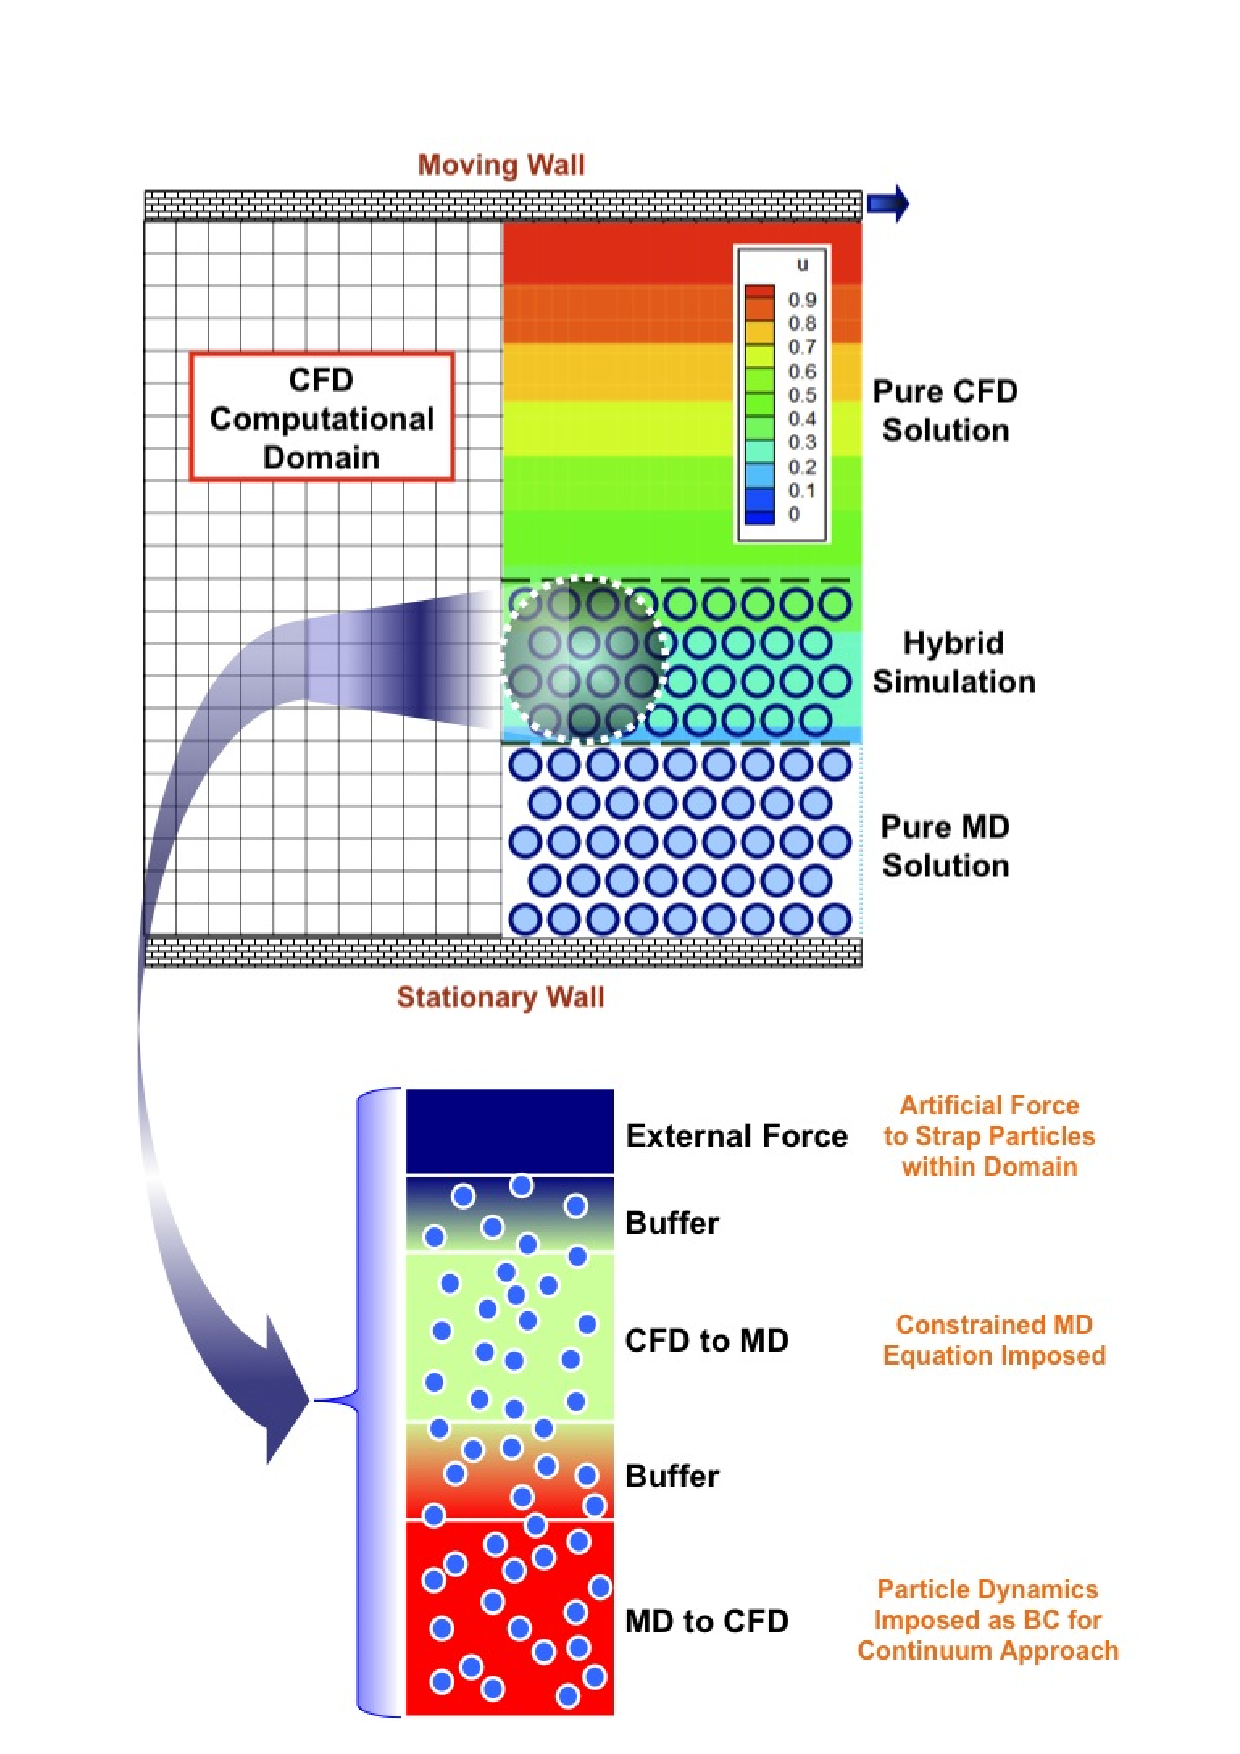
\includegraphics[scale=0.5]{fig1.pdf}
%\includegraphics[scale=0.3]{Couette7.pdf}
%\linebreak
\includegraphics[width=0.8\linewidth]{Couette7.pdf}
\vskip-0.2cm
\caption{Schematic Diagram of the Hybrid Domain with Detailed View of Overlapping Zone; Overall continuum/atomistic computational domain including overlap region is shown on left figure. Detailed layer by layer explanation of overlapping region is indicated by right figure.}
\label{Fig:Couette}
%\vspace{-1em}
\end{figure}
%%%%% FIGURE %%%%%



\section{IMPLEMENTATION OF HYBRID SCHEME ON CFD AND MD SOLVERS}

\subsection{Features of Baseline CFD and MD Codes}
Two-dimensional unsteady incompressible Navier-Stokes equations are chosen for governing equations to solve the nano-scale flow:

\vskip-.6cm
\begin{eqnarray}
\frac{\partial {u}_{i}}{\partial {x}_{i}} = 0
\end{eqnarray}
\vskip-.6cm
\begin{eqnarray}
\frac{\partial {u}_{i}}{\partial t} + \frac {\partial} {\partial {x}_{j}} ({u}_{i}{u}_{j}) = -\frac {\partial p} {\partial {x}_{j}} + \nu \frac {{\partial} {u}_{i}} {\partial {x}_{j} \partial {x}_{j}} \nonumber
\end{eqnarray}
where $\nu$ is the kinematic viscosity.

%The primary difficulty in solving the incompressible Navier-Stokes equations in primitive variables stems from the lack of a time derivative in the continuity equation. There is no straightforward way to iteratively march these equations in time and ensure a divergence-free velocity field.
%In this work, we adopted the pseudo-compressibility method$^{\cite{PseudoCompressibility}}$ to form a hyperbolic system of equations which can be marched in pseudo-time to a steady-state solution. The method can also be extended to solve time-dependent problems by using sub-iterations in pseudo-time at each physical time step. A time derivative of pressure is added to the continuity equation resulting in

In this work, we adopted the pseudo-compressibility method$^{\cite{PseudoCompressibility}}$ to form a hyperbolic system of equations which can be marched in pseudo-time. A time derivative of pressure is added to the continuity equation resulting in

\vskip-.6cm
\begin{eqnarray}
\frac{\partial (p/\rho)}{\partial \tau} = - \beta \frac{\partial {u}_{i}}{\partial {x}_{i}}
\end{eqnarray}
where $\beta$ denotes a pseudo-compressibility parameter, currently set up as 2.5.

For time-accurate unsteady simulation, dual time stepping method is adopted and it is combined with the LU-SGS (Lower-Upper Symmetric Gauss-Seidel) scheme$^{\cite{LU-SGS}}$ for the implicit time integration. The inviscid fluxes are upwind-differenced using Osher's flux-difference splitting scheme$^{\cite{Osher}}$. For higher-order spatial accuracy, the MUSCL (Monotone Upstream-centered Schemes for Conservation Laws)$^{\cite{MUSCL}}$ approach is used on inviscid flux calculation. Viscous fluxes are calculated using the conventional second-order central differencing.

Molecular dynamics (MD) a computer simulation technique is a specified computer simulation method for molecular systems, including microscopic details of a system and macroscopic statistical properties, which are the properties of the atoms, the interactions between particles, molecular characteristics, structure of molecules, transport phenomena etc.$^{\cite{Allen},\cite{Haile},\cite{Rapaport}}$ In molecular dynamics, an initial velocity is assigned to each atom, and Newton's laws are employed at the atomic level to propagate the system's motion through time evolution:

\vspace{-.2em}
%\footnotesize
\begin{equation}
F_{i} = m_{i}a_{i}
\label{eq:Newton}
\end{equation}
\normalsize
here each atom $\it i $ in a system constituted by N atoms, mi is the mass of i$^{th}$ atom, ai is the acceleration and denote by $\it {d^2r_{i}} / {dt^2}$, and $\it F_{i}$ is the force on i$^{th}$ atom, due to the atomic interaction which is calculated based on the potential energy between individual particles.
The simplest choice for the potential energy $\it U(r)$  can be written as the sum of pairwise interactions of particles:

\vspace{-.2em}
%\footnotesize
\begin{equation}
U(r_{1}, ...  ,r_{N}) =  \displaystyle\sum_{i} \displaystyle\sum_{j>i}  u(|r_{i} - r_{j}|)
\label{eq:PEnergy}
\end{equation}
\normalsize
where $\it i$ and $\it j$ particles are located at $r_{i}$ and $r_{j}$, and only $\it j>i$ cases have been considering for each particles pair once.
The most commonly used two-body interaction model is the Lennard-Jones (12-6) potential is applied to calculate pairwise interaction and is define as:

\vspace{-.2em}
%\footnotesize
\begin{equation}
 u(|r_{i} - r_{j}|) = 4\epsilon_{ij}[(\frac{\sigma_{ij}}{r_{ij}})^{12}-(\frac{\sigma_{ij}}{r_{ij}})^{6}]
 \label{eq:LJ12}
\end{equation}
\normalsize
where $\epsilon_{ij}$ and $\sigma_{ij}$ denote the pairwise potential well depth and the atom size parameter respectively, and $\it r_{ij}$ is the distance between the particle $\it i$ and $\it j$.
The term $\it 1/r_{ij}^{12}$ dominating at short range distance repulsive behavior based on the Pauli principle to avoid overlapping the electronic clouds when particles are  brought very close to each other. The term $\it 1/r_{ij}^6$ dominates at long range attractive forces by van der Waals dispersion forces.

The time integration algorithm is required to integrate the equation of motion of the interacting particles and computing molecular trajectories, one of most common velocity Verlet algorithm is employed to compute the simulation.
In this work,  the MD simulations were performed by using the modified version of Large Atomic Molecular Massively Parallel Simulator(LAMMPS). It is the classical molecular dynamics open software written in C++ and developed by Sandia National Labs $\underline{(http://lammps.sandia.gov/)}$.



\subsection{Implementation of Hybrid Scheme}
CFD-MD hybrid method has numerical strategy for file-based information exchange between continuum description for macroscopic scale and discrete particle description for microscopic scale. For this information exchange, both codes have the file interface, where each writes the velocity profile of overlapping region, waits for its counterpart's velocity data and receive the data as a boundary condition in the overlap region.

Additional change made on CFD code is the implementation of overlapping scheme, in the same way as Chimera overset mesh$^{\cite{Chimera}}$. That is, pure MD region is declared as holes and MD boundary layers are treated as fringe cells.

On the other hands, MD code experiences a lot of change to implement hybrid scheme. First, the external force should be imposed to prevent leaving particles from the control domain and the force is applied its perpendicular relative position of uppermost MD layer.

\vspace{-.2em}
%\footnotesize
\begin{equation}
 F_{ext, i} = -p_{a}\sigma\frac{y_{i}-Y_{n-1}}{1-(y_{i}-Y_{n-1})/(Y_{n}-Y_{n-1})}
 \label{eq:Con_vel}
\end{equation}
\normalsize
where $\it p_{a}$ denote the average pressure in the MD region, $\it Y_{n}-Y_{n-1}$ is the thickness of the uppermost layer which is applied the force and $\it F_{ext}$ is the external force acting on $\it i_{th}$ particle located on position $\it y_{i}$.

Communicate MD information to CFD can be achieved uncomplicated since the coarse grained microscopic information in time is imposed to macroscopic resolution of the continuum domain. The reverse procedure, to implement  CFD to MD communication, is more difficult and requires artificial intervention to maintain mass and momentum conservation. The average velocities of particles in $\it J_{th}$ cell is equal to the velocity $\it u_{J}$ in continuum cell.

\vspace{-.2em}
%\footnotesize
\begin{equation}
 u_{J}(t) = \frac{1}{N_{J}} \displaystyle\sum_{i} v_{i}
 \label{eq:Con_vel}
\end{equation}
\normalsize
where $\it v_{i}$ is velocity of  $\it i_{th}$ particle and $\it N_{J}$ is the number of particles in the cell.   With taking Lagrangian derivative  of eq.~\ref{eq:Con_vel},

\vspace{-.2em}
%\footnotesize
\begin{equation}
 \frac{Du_{J}(t)}{Dt} =  \displaystyle\sum_{i} \frac{\ddot{x_{i}}}{N_{J}}
 \label{eq:Lagrangian}
\end{equation}
\normalsize
The Classical MD equation of motion can be generalized to obtain constraint by adopting the fluctuation in acceleration of each particles, $\zeta_{i}$

\vspace{-.2em}
%\footnotesize
\begin{equation}
 \frac{F_{i}}{m_{i}} = \ddot{x_{i}}(t)  =   \frac{Du_{J}(t)}{Dt} + \zeta_{i} = \frac{\displaystyle\sum_{i}F_{i}(t)} {\displaystyle\sum_{i}m_{i}} +   \zeta_{i}
 \label{eq:Con2}
\end{equation}
\normalsize
where $\it F_{i}$ is the force on $\it i_{th}$ particle based on the interactions between particles,  $\it m_{i}$ is mass of each atom and  eq.~\ref{eq:Con2} satisfies,
\vspace{-.2em}
%\footnotesize
\begin{equation}
\displaystyle\sum_{i}\zeta_{i}m_{i} = 0
 \label{eq:Con2}
\end{equation}
\normalsize
The constrained particle dynamics with conventional equation of motion can be written as:

\vspace{-.2em}
%\footnotesize
\begin{equation}
 \ddot{x_{i}}(t) = \frac{F_{i}}{m_{i}} -  \frac{\displaystyle\sum_{i}F_{i}(t)} {\displaystyle\sum_{i}m_{i}} - \frac{1}{\Delta t_{MD}} \{  \frac{\displaystyle\sum_{i}m_{i}\dot{x_{i}}} {\displaystyle\sum_{i}m_{i}} - u_{J}(t + \Delta t_{MD})\}
 \label{eq:Con3}
\end{equation}
\normalsize
The continuum velocity and the mean microscopic velocity from MD over control domain provide the synchronization of the mass and momentum consistent via eq.~\ref{eq:Con3}.



Figure~\ref{Hybrid_Timescale} shows the schematic view of synchronization mechanism between CFD and MD domains. When both solvers approach the data exchange point (denoted by $t-{\Delta}t$), they exchange the information in the overlapping region and advance to the next exchange point ($t$). In the data exchange point, CFD sends the velocity profile at that instance. On the other hand, MD sends averaged velocity over a finite time duration ($S_{MD}{\times}{\Delta}t$). In MD simulation, spatially averaged velocity at an instance contains very high noise, thus it is inevitable to average particles' velocities over time. Data exchange interval (${\Delta}t$) is set sufficiently large compared to the averaging duration.

This mechanism gives us a better parallel efficiency compared to conventional sequential coupling mechanisms where one domain advances to the next exchange point and leads its counterpart to approach this point.$^{\cite{Time_Mechanism}}$ As they send and receive their flow data at the same point, both codes can independently advance to the next time level without a large computing cost on waiting. So, parallel performance can ideally reach the single code running only if an appropriate load balancing between two domains can be applied. However, we should agree that this approach inherently includes the time lagging in CFD-MD boundary zone, because averaged molecular dynamic velocity over backward time scale is represented as the solution at that instance.
% Additionally, in any algorithm, codes experience the time lagging due to the impose of explicit BC in the hybrid domain.

\begin{figure}[ht]
\centering
\includegraphics[width=0.7\linewidth]{Hybrid_Flowchart_1.pdf}
\vskip-0.2cm
\caption{Time Evolution Mechanism of Application Codes; CFD and MD codes are scheduled to conduct data exchange in the overlapping region at every $\Delta{t}$ time. CFD and MD solvers do sub-iterations until approaching the next data exchange point, by $I_{CFD}$ and $I_{MD}$. CFD solution at $t-\Delta{t}$ is directly applied as the boundary condition for MD simulation from $t-\Delta{t}$ to $t$, while averaged molecular dynamic velocity on $S_{MD}\times\Delta{t_{MD}}$ durations are imposed as CFD boundary conditions at this time instance.}
\label{Hybrid_Timescale}
\end{figure}



% Figure~\ref{Hybrid_Flowchart} denotes overall flowchart of CFD and MD solvers. Until they reach the file exchange point, both codes independently run their solution procudure. At the data exchange point, both codes first send the data and wait for receiving.

%
%\begin{figure}[ht]
%\centering
%\includegraphics[width=0.6\linewidth]{Hybrid_Flowchart_2.pdf}
%\vskip-0.2cm
%\caption{Flowchart of Coupled Codes; CFD and MD codes have the identical flowchart except the information exchange between two codes and the additional consideration of a hybrid boundary condition. On every data exchange period, both codes first write their flow properties in the hybrid region and wait for the datafile from their counterpart. As they exchange their flow data at the same time level, they can concurrently advance to the next time level without a large computing cost on waiting for data exchange.}
%\label{Hybrid_Flowchart}
%\end{figure}



\section{NUMERICAL RESULTS}

\subsection{Validation and Verification of a Coupled Simulation Package}
The first problem is the Couette flow simulation, which have been in wide use for the validation of a hybrid CFD-MD solver.$^{\cite{Nie},\cite{Yen}}$ We start from the validation case, which has 52$\sigma$ distance between two parallel plates and upper wall velocity is ${\sigma}/{\tau}$. We assume liquid argon particles are filled in the domain and both walls have artificial properties which is the same as those of liquid argon. Characteristic length of liquid argon is ${\sigma}=3.405{\times}10^{-10}$ and time scale is $\tau=2.2{\times}10^{-12}$. Density is $0.81m{\sigma}^{-3}$, which means 0.81 atoms are included in the characteristic volume.

As we have argued eariler, MD solution inherently describes the fluctuating pattern of particles, which becomes a noise in CFD solution. Thus, the first thing to do for coupled simulation is to decide coupling conditions including layer size, sampling duration, sampling interval and MD timescale, which defines the scale and pattern of noise. For continuum approach, averaging more particles on bigger layers for a long time would be preferred to eliminate the systematic noise of molecular vibration. However, in view of MD, smaller layer is preferred to accurately apply the velocity gradient from CFD solution. Also, longer sampling duration and the resulting longer sampling interval will increase the time-lagging in hybrid boundary. Thus, quantitative consideration on optimal scaling of these conditions are highly required.

Figure \ref{MD_Regular_Vel0} shows the fluctuation of averaged velocity in pure MD simulations of stationary flow. Domain size is the same as our validation problem and this domain is split to 6, 12, 24, 48 layers in Y-direction to compute the flow velocity. As the flow is stationary, all averaged velocities should be zero regardless of the number of layers. However, the L2 norm of averaged velocity tends to increase with more layers (from 6 to 48), meaning that bigger layer size is required to reduce the noise in hybrid boundary. The strength of fluctuation converges to 0.01$\sigma$/$\tau$ as we increase the sampling interval, which implies that the fluctuation of $\pm$0.01 in hybrid boundary is unavoidable. The fluctuation did not decrease with smaller MD timescale and this concludes us that this fluctuation and its scale is physically natural phenomenon. From this test, we decide the coupling condition as $\Delta{t_{MD}}=5\times{10^{3}}$ with each layer size to be 2$\sigma$ (which is nearly equivalent to having 24 layer), sampling duration of 10$\tau$ and sampling interval is set up the double of sampling duration.

%
\begin{figure}[ht]
\centering
\includegraphics[width=0.4\linewidth]{MD_Regular_Vel0_5e-3.pdf}
\hskip 1cm
\includegraphics[width=0.4\linewidth]{MD_Regular_Vel0_1e-3.pdf}
\vskip-0.2cm
\caption{L2 Norm of Averaged Velocity with Different Layer Sizes and Sampling Duration, at $\Delta{t_{MD}}=5\times{10^{3}}$ (Left) and $\Delta{t_{MD}}=1\times{10^{3}}$ (Right); Solution tends to produce less noise with bigger layer size and smaller MD timescale in short sampling duration. As sampling interval is increased, all solutions converges to the same fluctuation strength, which is 0.01$\sigma/\tau$.}
\label{MD_Regular_Vel0}
\end{figure}



Resulting CFD and MD computational domains are depicted in Fig.~\ref{Couette_Val_Domain}. In CFD mesh, the cell size in Y-direction is 2$\sigma$. Pure MD region is specified to be 10$\sigma$, which was observed to be sufficient to prevent strong fluctuation between fluid particles and wall materials from directly transported to CFD domains by iterative testruns. Two layer boundary zones from particle to continuum domain is placed ahead of pure MD region, from 10 to 14$\sigma$. Continuum to particle boundary is positioned from 18 to 22$\sigma$ and external force region is place at the top of hybrid region, from 24 to 26$\sigma$. MD domain has sufficiently large length in the principal flow direction, to include enough number of particles in the hybrid data average region.

%
\begin{figure}[ht]
\centering
\includegraphics[width=0.6\linewidth]{Couette_Val_Domain.pdf}
\vskip-0.2cm
\caption{Computational Domain of Couette Flow Simulation; The height of the fluid domain is 52$\sigma$ ($\approx$177$\AA$). CFD mesh size is 201$\times$27 and CFD cells at the pure MD region are treated as holes. MD domain size is about 210$\sigma$ in the X-direction and around 30$\sigma$ in the Y-direction, including the bottom wall. Periodic boundary condition is applied on the principal flow direction.}
\label{Couette_Val_Domain}
\end{figure}



Unsteady Couette flow profile by CFD, MD and hybrid simulations are presented in Fig.~\ref{Flat_Plate_Sol}. Pure CFD produces identically the same result as analytic solution and MD simulations also describes the same flow physics. In MD simulation, fluctuating pattern is observed during the evolution. This causes the slight variation in hybrid solution, along with the time-lagging in current algorithm. After convergence, the solution follows the same flow pattern as steady profile, which proves that the hybrid approach can accurately analyze the steady flow profile in micro-scaled systems.

%
\begin{figure}[ht]
\centering
\includegraphics[width=0.4\linewidth]{Flat_Plate_Sol1.pdf}
\hskip 1cm
\includegraphics[width=0.4\linewidth]{Flat_Plate_Sol2.pdf}
\vskip-0.2cm
\caption{Unsteady Couette Flow Profile; (Left) Pure CFD solution is exactly the same as analytic solution. MD solution shows the same flow pattern as analytic solution, though some fluctuation is observed. This verifies that CFD and MD represents the same flow physics. (Right) The steady result by hybrid approach produces the same numerical result as analytic solution, though the time-lagging in the hybrid boundary is observed during the evolution.}
\label{Flat_Plate_Sol}
\end{figure}



The same domain with coupling condition is applied to solve the Stokes boundary layer problem, which is purely unsteady problem. In this case, the upper wall boundary condition changes from the fixed velocity to oscillatory wall, which is $u_{wall}(t)=({\sigma}/{\tau}){\times}sin(2{\pi}t/T)$. Period $T$ is set 200$\tau$. Velocity in the hybrid region becomes far slower than the Couette flow profile, so the influence of noise from MD side is concerned to be more critical in the current flow simulation.

Figure~\ref{Stokes_Sol} shows the oscillatory velocity profile by pure CFD and hybrid simulations. Unsteady profile in both simulations are globally the same, proving that the current approach can be directly applied to unsteady problems. In detail, fluctuation in MD domain is not so strong in hybrid region. Though minor time-lagging profile is seen from MD solution, this does not change the global flow profile dominantly because the driving force in this simulation is the oscillating velocity from CFD domain.

%
\begin{figure}[ht]
\centering
\includegraphics[width=0.4\linewidth]{Stokes_Sol_1.pdf}
\hskip 1cm
\includegraphics[width=0.4\linewidth]{Stokes_Sol_2.pdf}
\vskip-0.2cm
\caption{Unsteady Flow Profile of Stokes Boundary Layer Problem; Solution by pure CFD simulation is denoted by a solid line and solution by hybrid simulation is presented by symbols. Hybrid flow profile globally matches well with CFD solution, though slight time-lagging in the MD side is observed. This evaluates that current hybrid approach can be applied to purely unsteady problem.}
\label{Stokes_Sol}
\end{figure}



\subsection{Application to Realistic System}

%(Changed problem size with changed hybrid condition; 1 paragraph)\\
To be included\\




\section{CONCLUSIONS}
(Summarizing; 1 paragraph)\\

(Our limitation and future works; 1 paragraph)\\



\section*{ACKNOWLEDGEMENT}
This work is part of the Cybertools (\underline {http://cybertools.loni.org/}) project and primarily funded by NSF/LEQSF (2007-10)-CyberRII-01.
%This work has also been made possible thanks to computer resources provided by LONI.


\begin{thebibliography}{99}
%\bibitem{Zienkiewicz} O. C. Zienkiewicz and R. C. Taylor, The finite element method, 4th Edition, \textit{McGraw Hill}, \textbf{Vol. I} (1989), \textbf{Vol. II} (1991).
%\bibitem{Idelsohn} S. Idelsohn and E. O\~nate, Finite element and finite volumes, Two good friends, \textit{Int. J. Num. Meth. Engng.}, \textbf{37}, 3323--3341 (1994).
%\bibitem{Abgrall} R. Abgrall, M. Ricchiuto, N. Villedieu, C. Tav\'e\ and H. Deconinck, Very High Order Residual Distribution On Triangular Grids, In proceedings of the \textit{European Conference on Computational Fluid Dynamics}, ECCOMAS CFD 2006, P. Wesseling, E. O\~nate and J. Periaux Eds., Egmond aan Zee, Netherlands, Paper n$^{\circ}$583 (2006)



\bibitem{Thompson} S.T. O'Connell and P.A. Thompson, Molecular Dynamics Continuum Hybrid Computations: a Tool for Studying Complex Fuid Flows, \textit{Phys. Rev. E.}, \textbf{500}, 55--64 {2004}.
\bibitem{Nie} X. B. Nie and S. Y. Chen, W. N. E and M. O. Robbins, A Continuum and Molecular Dynamics Hybrid Method for Micro- and Nano-Fluid Flow, \textit{J. Fluid Mech.}, \textbf{52}, R5792--R5795 {1995}.
\bibitem{Yen} T. H. Yen and C. Y. Soong and P. Y. Tzeng, Hybrid Molecular Dynamics-Continuum Simulation for Nano/Mesoscale Channel Flow, \textit{Microfluid Nanofluid}, \textbf{3}, 665--675 {2007}.
\bibitem{Steijl} R. Steijl and G. N. Barakos, Coupled Navier-Stokes--Molecular Dynamics Simulations using a Multi-physics Flow Simulation Framework, \textit{Int. J. Numer. Meth. Fluids}, \textbf{62}, 1081--1106, {2010}
\bibitem{CCGrid} S.-H. Ko, N. Kim, J. Kim, A. Thota and S. Jha, Efficient Runtime Environment for Coupled Multi-Physics Simulations: Dynamic Resource Allocation and Load-Balancing, In proceedings of \textit{The 10th IEEE/ACM International Symposium on Cluster, Cloud and Grid Computing (CCGrid 2010)}, Accepted for Publication {2010}

\bibitem{Flekkoy} E. G. Flekk$\phi$y, G. Wagner and J. Feder, Hybrid Model for Combined Particle and Continuum Dynamics., \textit{Europhys Lett.}, \textbf{52}, 271--276 {2000}.
\bibitem{Wagner} G. Wagner, E. G. Flekkoy, J. Feder, T. Jossang, Coupling molecular dynamics and continuum dynamics., \textit{Comput. Phys. Commun.}, \textbf{147}, 670--673 {2002}.
\bibitem{Hadjicon1} N. G. Hadjiconstantinou, A. T. Patera., Heterogeneous Atomistic Continuum Representations for Dense Fluid Systems., \textit{ Int. J. Mod. Phy.}, \textbf{4},  967--976 {1997}.
\bibitem{Hadjicon2} N. G. Hadjiconstantinou, A. L. Garcia, M. Z. Bazant, G. He, Statistical Error in Particle Simulations of Hydrodynamic Phenomena., \textit{J. Comput. Phys.}, \textbf{187}, 274--297 {2003}.
\bibitem{Wang} Y. C. Wang, G. He, A Dynamic Coupling Model for Hybrid Atomistic-Continuum Computations., \textit{Chem. Eng. Sci.}, \textbf{62}, 3574--3579 {2007}.

\bibitem{PseudoCompressibility} S. E. Rosers and D. Kwak, An Upwind Differecing Scheme for the Time-Accurate Incompressible Navier-Stokes Equations, \textit{AIAA J.}, \textbf{28}, 253--262 {1990}.
\bibitem{LU-SGS} S. Yoon and A. Jameson, Lower-Upper Symmetric-Gauss-Seidel Method for the Euler and Navier-Stokes Equations, \textit{AIAA J.}, \textbf{26}, 1025--1026 {1988}.
\bibitem{Osher} M. M. Rai and S. R. Chakaravarthy, An Implicit Form of the Osher Upwind Scheme, \textit{AIAA J.}, \textbf{24}, 735--743 {1986}.
\bibitem{MUSCL} B. Van Leer, Towards the Ultimate Conservative Difference Scheme. V. A Second Order Sequel to Godunov's Methods, \textit{J. Comp. Phys.}, \textbf{32}, 101--136 {1979}.
\bibitem{Allen} M. Allen and D. Tildesley, Computer Simulation of Liquids, \textit{Oxford. Science Publications }, {1987}.
\bibitem{Haile}  J. M. Haile, Molecular Dynamics Simulation. Elementary Methods, \textit{Wiley, Chichester}, {1992}.
\bibitem{Rapaport} D C. Rapaport, The Art of Motecutar Dynamics Simulation, \textit{Cambridge University Press}, {1995}.

\bibitem{Chimera} J. L. Steger, F. C. Dougherty and J. A. Benek, A Chimera Grid Scheme, \textit{Advances in Grid Generation}, \textbf{FED Vol. 5}, American Society of Mechanical Engineers, New York, 59?-69 {1983}.
\bibitem{Time_Mechanism} R. Delgado-Buscalioni and P. V. Coveney, Hybrid Molecular-Continuum Fluid Dynamics, \textit{Phil. Trans. R. Soc. Lond. A}, \textbf{362}, 1639--1654 {2004}.

\end{thebibliography}



\end{document}

